\chapter{System Architecture and Design}
\label{chap:system_architecture}

\section{System Overview and Architectural Paradigm}
\label{sec:arch_overview}

ChronaNexus is engineered as a decoupled, multi-tier clinical intelligence platform designed to ingest multi-source, multi-year medical records and provide auditable, real-time clinical decision support. The architectural paradigm is anchored upon three fundamental design principles:
\begin{enumerate}
    \item \textbf{Asymmetric Hybrid Processing}: The system cleanly separates unstructured linguistic summarization (handled by local Small Language Models or cloud LLMs) from deterministic mathematical aggregation and temporal reasoning (handled by an ACID relational database and symbolic rule interceptors). This prevents the language model from hallucinating numerical values or reversing chronological sequences.
    \item \textbf{Fail-Closed Verification Loop}: Every clinical response generated by the reasoning engine is intercepted by an autonomous evidence grounding verifier. Rather than trusting model self-evaluation, the verifier decomposes the response into atomic propositions, compares them against retrieved context passages, and purges ungrounded assertions before the response reaches the user interface.
    \item \textbf{Local-First Edge Execution}: To guarantee patient data sovereignty under healthcare privacy regulations (such as the DPDP Act 2023~\cite{nha2022abdm}), the system runtime is fully self-contained. The backend operates on lightweight local embeddings (\texttt{bge-small-en-v1.5}), an embedded vector store (\texttt{ChromaDB}), an ACID relational store (\texttt{SQLite}), and an offline Small Language Model running on CPU hardware.
\end{enumerate}


\section{3-Tier Physical Architecture}
\label{sec:arch_3tier}

The platform follows a classic 3-Tier Physical Architecture comprising the Presentation Tier, Application Tier, and Data and Knowledge Tier. Figure~\ref{fig:4_1_architecture} provides the detailed architectural schematic.

\begin{figure}[htbp]
    \centering
    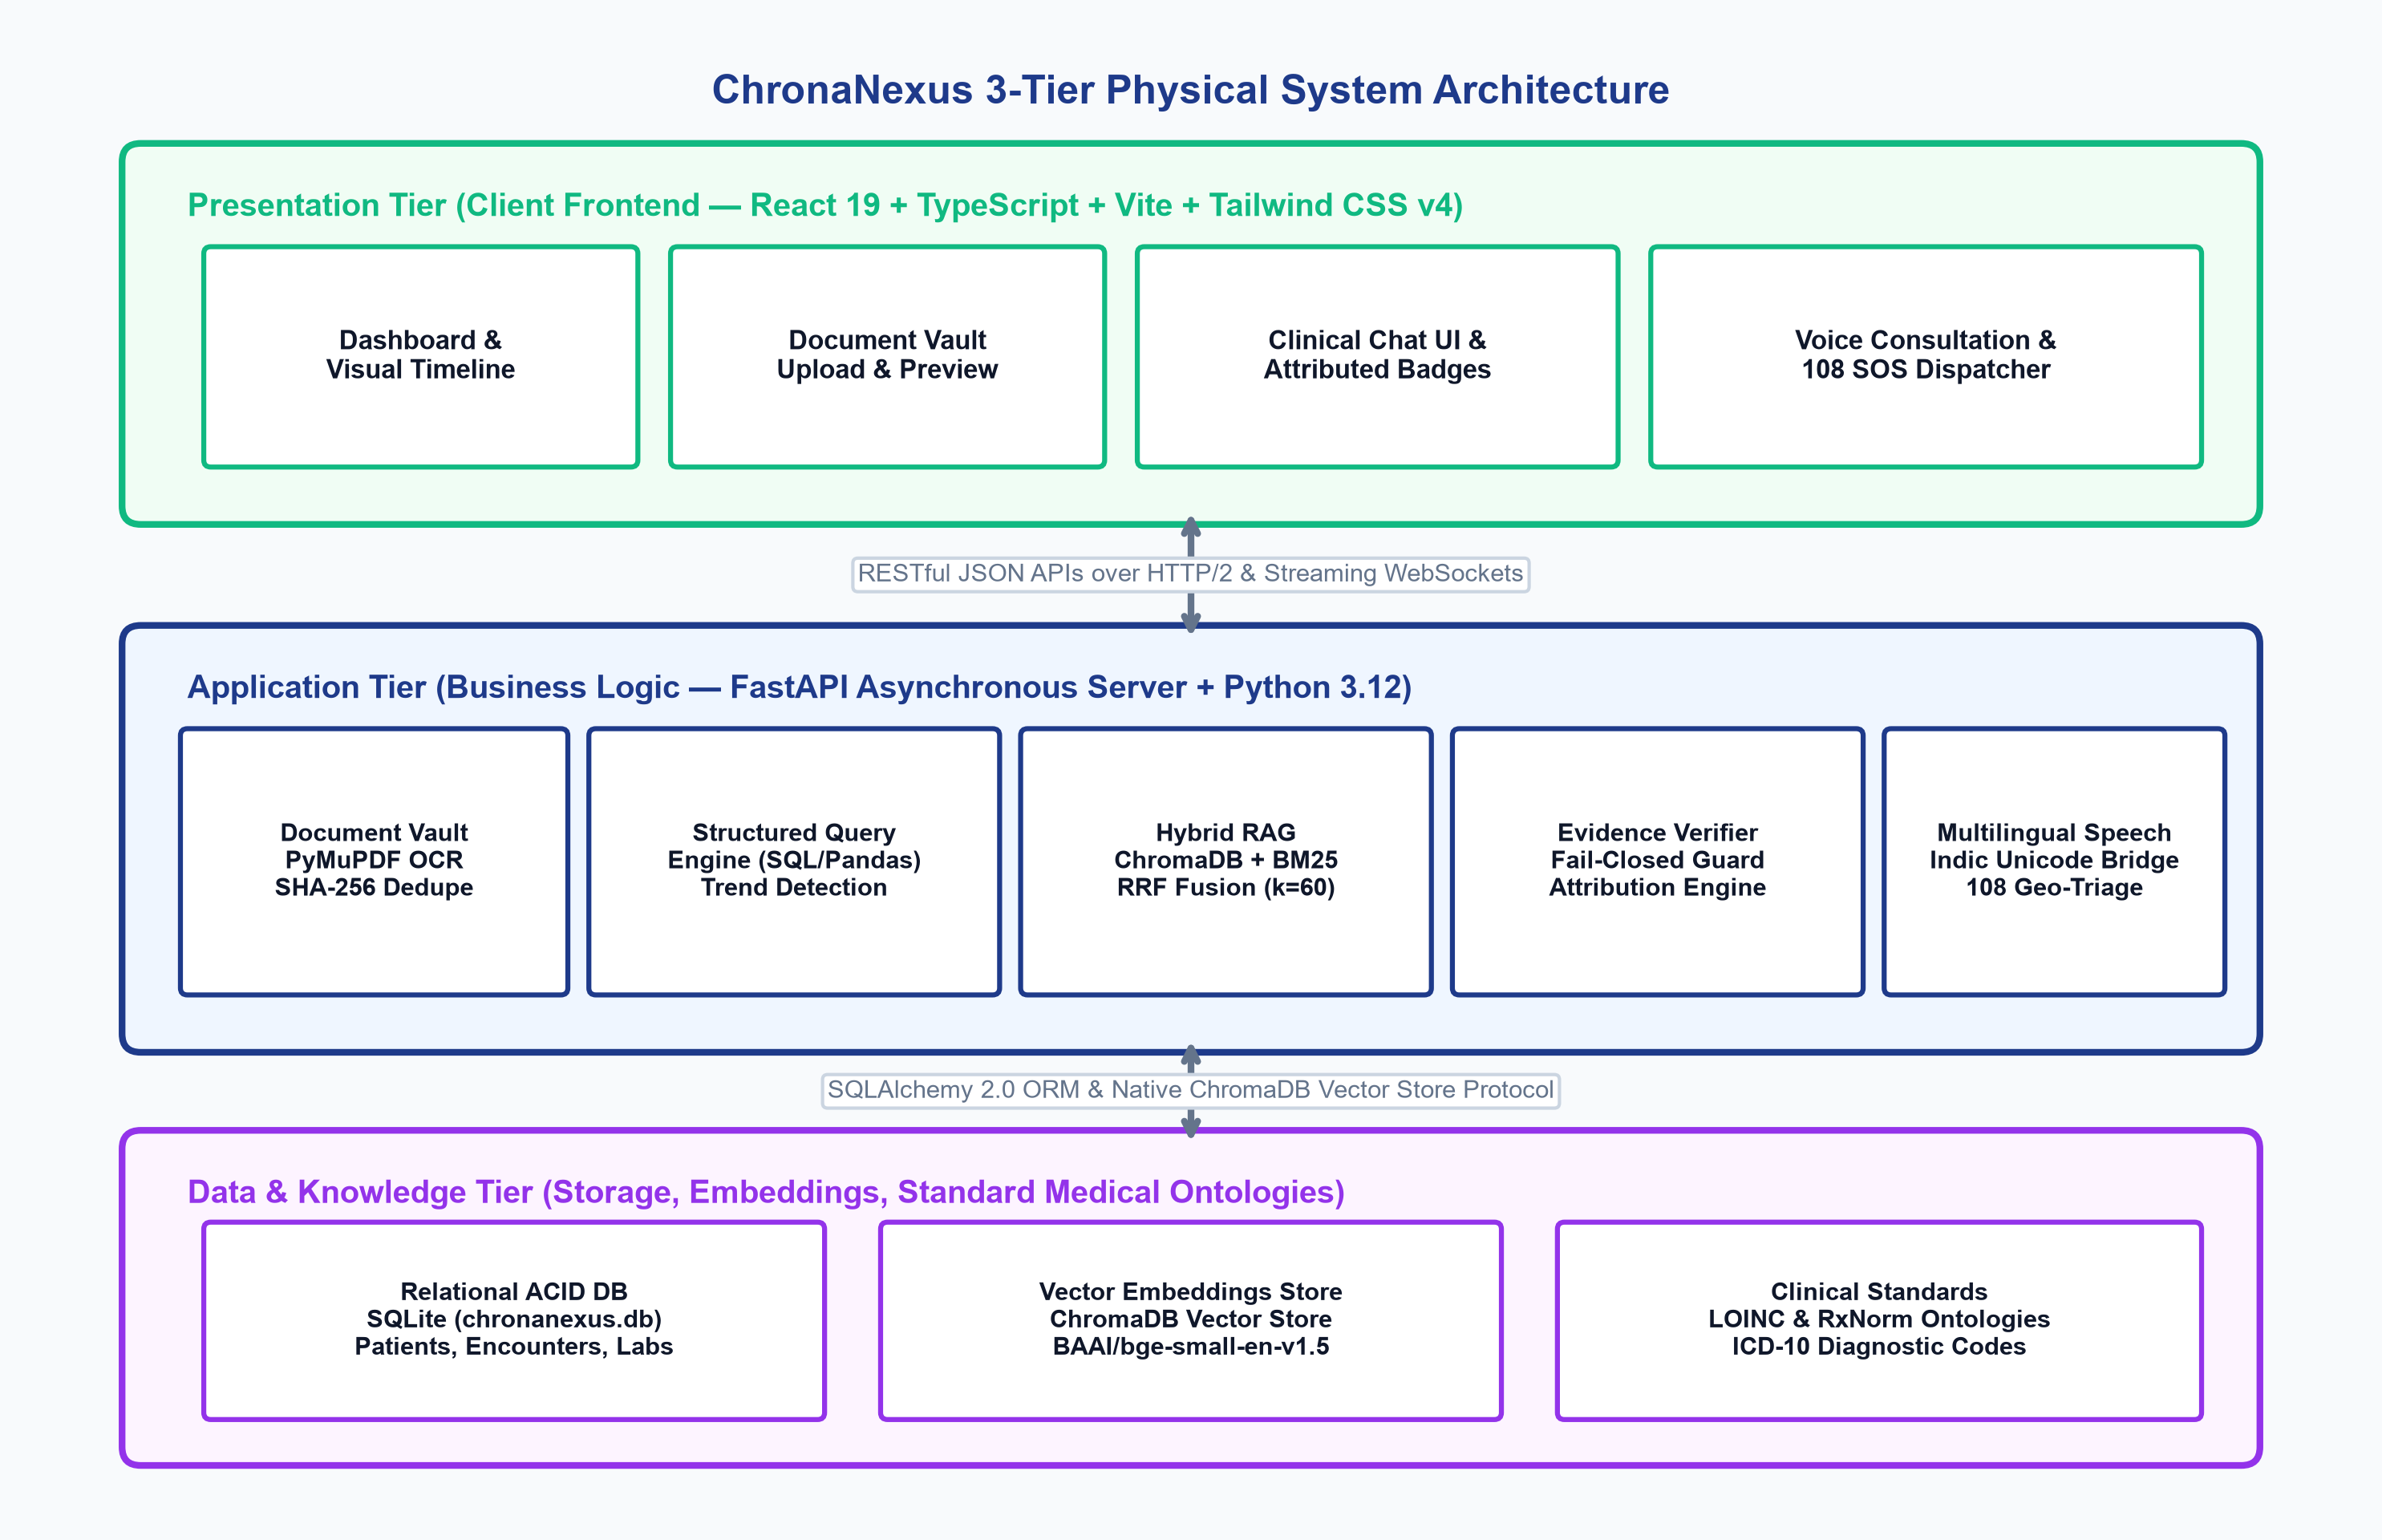
\includegraphics[width=0.95\linewidth]{figures/fig4_1_architecture.png}
    \caption{ChronaNexus 3-Tier Physical System Architecture illustrating components and data buses.}
    \label{fig:4_1_architecture}
\end{figure}

\subsection{Tier 1: Presentation Tier (Client Frontend)}
The user interface is engineered as a high-performance single-page application (SPA) utilizing \textbf{React 19}, \textbf{TypeScript}, and \textbf{Vite}. The visual styling leverages \textbf{Tailwind CSS v4} to implement an accessible clinical glassmorphism design system. Key frontend components include:
\begin{itemize}
    \item \textbf{Longitudinal Timeline Explorer}: Interactive visual chronometer rendering multi-year encounters (2019--2026) with facility badges, clinical tags, and collapsible document previews.
    \item \textbf{Dynamic Laboratory Trend Charts}: Responsive SVG visualizers plotting numerical lab analytes (e.g., Fasting Glucose, HbA1c, Serum Creatinine) across time with physiological normal reference bands.
    \item \textbf{Auditable Clinical Chat Console}: Real-time conversational interface supporting Server-Sent Events (SSE) streaming, rendering clickable citation badges linked directly to underlying source document pages.
    \item \textbf{Multilingual Voice Assistant \& SOS Triage}: Audio capture and streaming player with native Indic language selection, waveform feedback, and one-click emergency dispatch triggering.
\end{itemize}

\subsection{Tier 2: Application Tier (Business Logic Gateway)}
The middle tier is powered by an asynchronous \textbf{FastAPI} server written in \textbf{Python 3.12}, hosted via \textbf{Uvicorn}. It exposes versioned RESTful JSON endpoints alongside streaming WebSockets. This tier coordinates five discrete micro-services:
\begin{enumerate}
    \item \textbf{Document Vault \& Extraction Service}: Manages multipart file uploads, executes SHA-256 binary deduplication, and invokes \texttt{PyMuPDF} for layout-aware table extraction.
    \item \textbf{Structured Query \& Timeline Engine}: Translates temporal inquiries into parameterized SQL queries against the relational store, computing chronological deltas ($\Delta = V_t - V_{t-1}$) without model hallucination.
    \item \textbf{Dual-Channel Hybrid Retrieval Service}: Coordinates parallel dense vector search (\texttt{ChromaDB}) and exact lexical search (\texttt{BM25 Okapi}), aggregating results via Reciprocal Rank Fusion ($k=60$).
    \item \textbf{Evidence Grounding \& Claim Verifier}: Parses draft responses into atomic propositions, evaluating them through Tier 1 symbolic regex rules and Tier 2 neural natural language inference.
    \item \textbf{Indic Speech \& Emergency Dispatch Service}: Implements the Unicode phonetic transliteration bridge ($\Delta = -0x0180$) for Odia voice synthesis and coordinates emergency geolocation via OpenStreetMap Overpass API.
\end{enumerate}

\subsection{Tier 3: Data and Knowledge Tier (Storage \& Ontologies)}
The persistence tier provides robust, ACID-compliant relational storage combined with an embedded vector index:
\begin{itemize}
    \item \textbf{Relational Database (\texttt{SQLite} / \texttt{SQLAlchemy 2.0})}: Stores structured patient demographics, clinical encounters, standardized laboratory analytes, active medications, chat session histories, and immutable verification audit logs.
    \item \textbf{Vector Store (\texttt{ChromaDB})}: Stores $384$-dimensional dense vector embeddings generated by \texttt{BAAI/bge-small-en-v1.5}~\cite{xiao2023bge}, partitioned by patient identifier to ensure complete multi-tenant tenant isolation.
    \item \textbf{Standard Clinical Ontologies}: Embedded lookup catalogs mapping raw clinical terminology to canonical LOINC (laboratory observations), RxNorm (active pharmacotherapy), and ICD-10 (diagnoses) codes.
\end{itemize}


\section{Data Flow Modeling}
\label{sec:arch_dfd}

The flow of clinical intelligence through the system is formally specified through Data Flow Diagrams. Figure~\ref{fig:4_2_dfd} illustrates the Level-1 Data Flow Diagram (DFD), delineating external entities, primary processing kernels, and data repositories.

\begin{figure}[htbp]
    \centering
    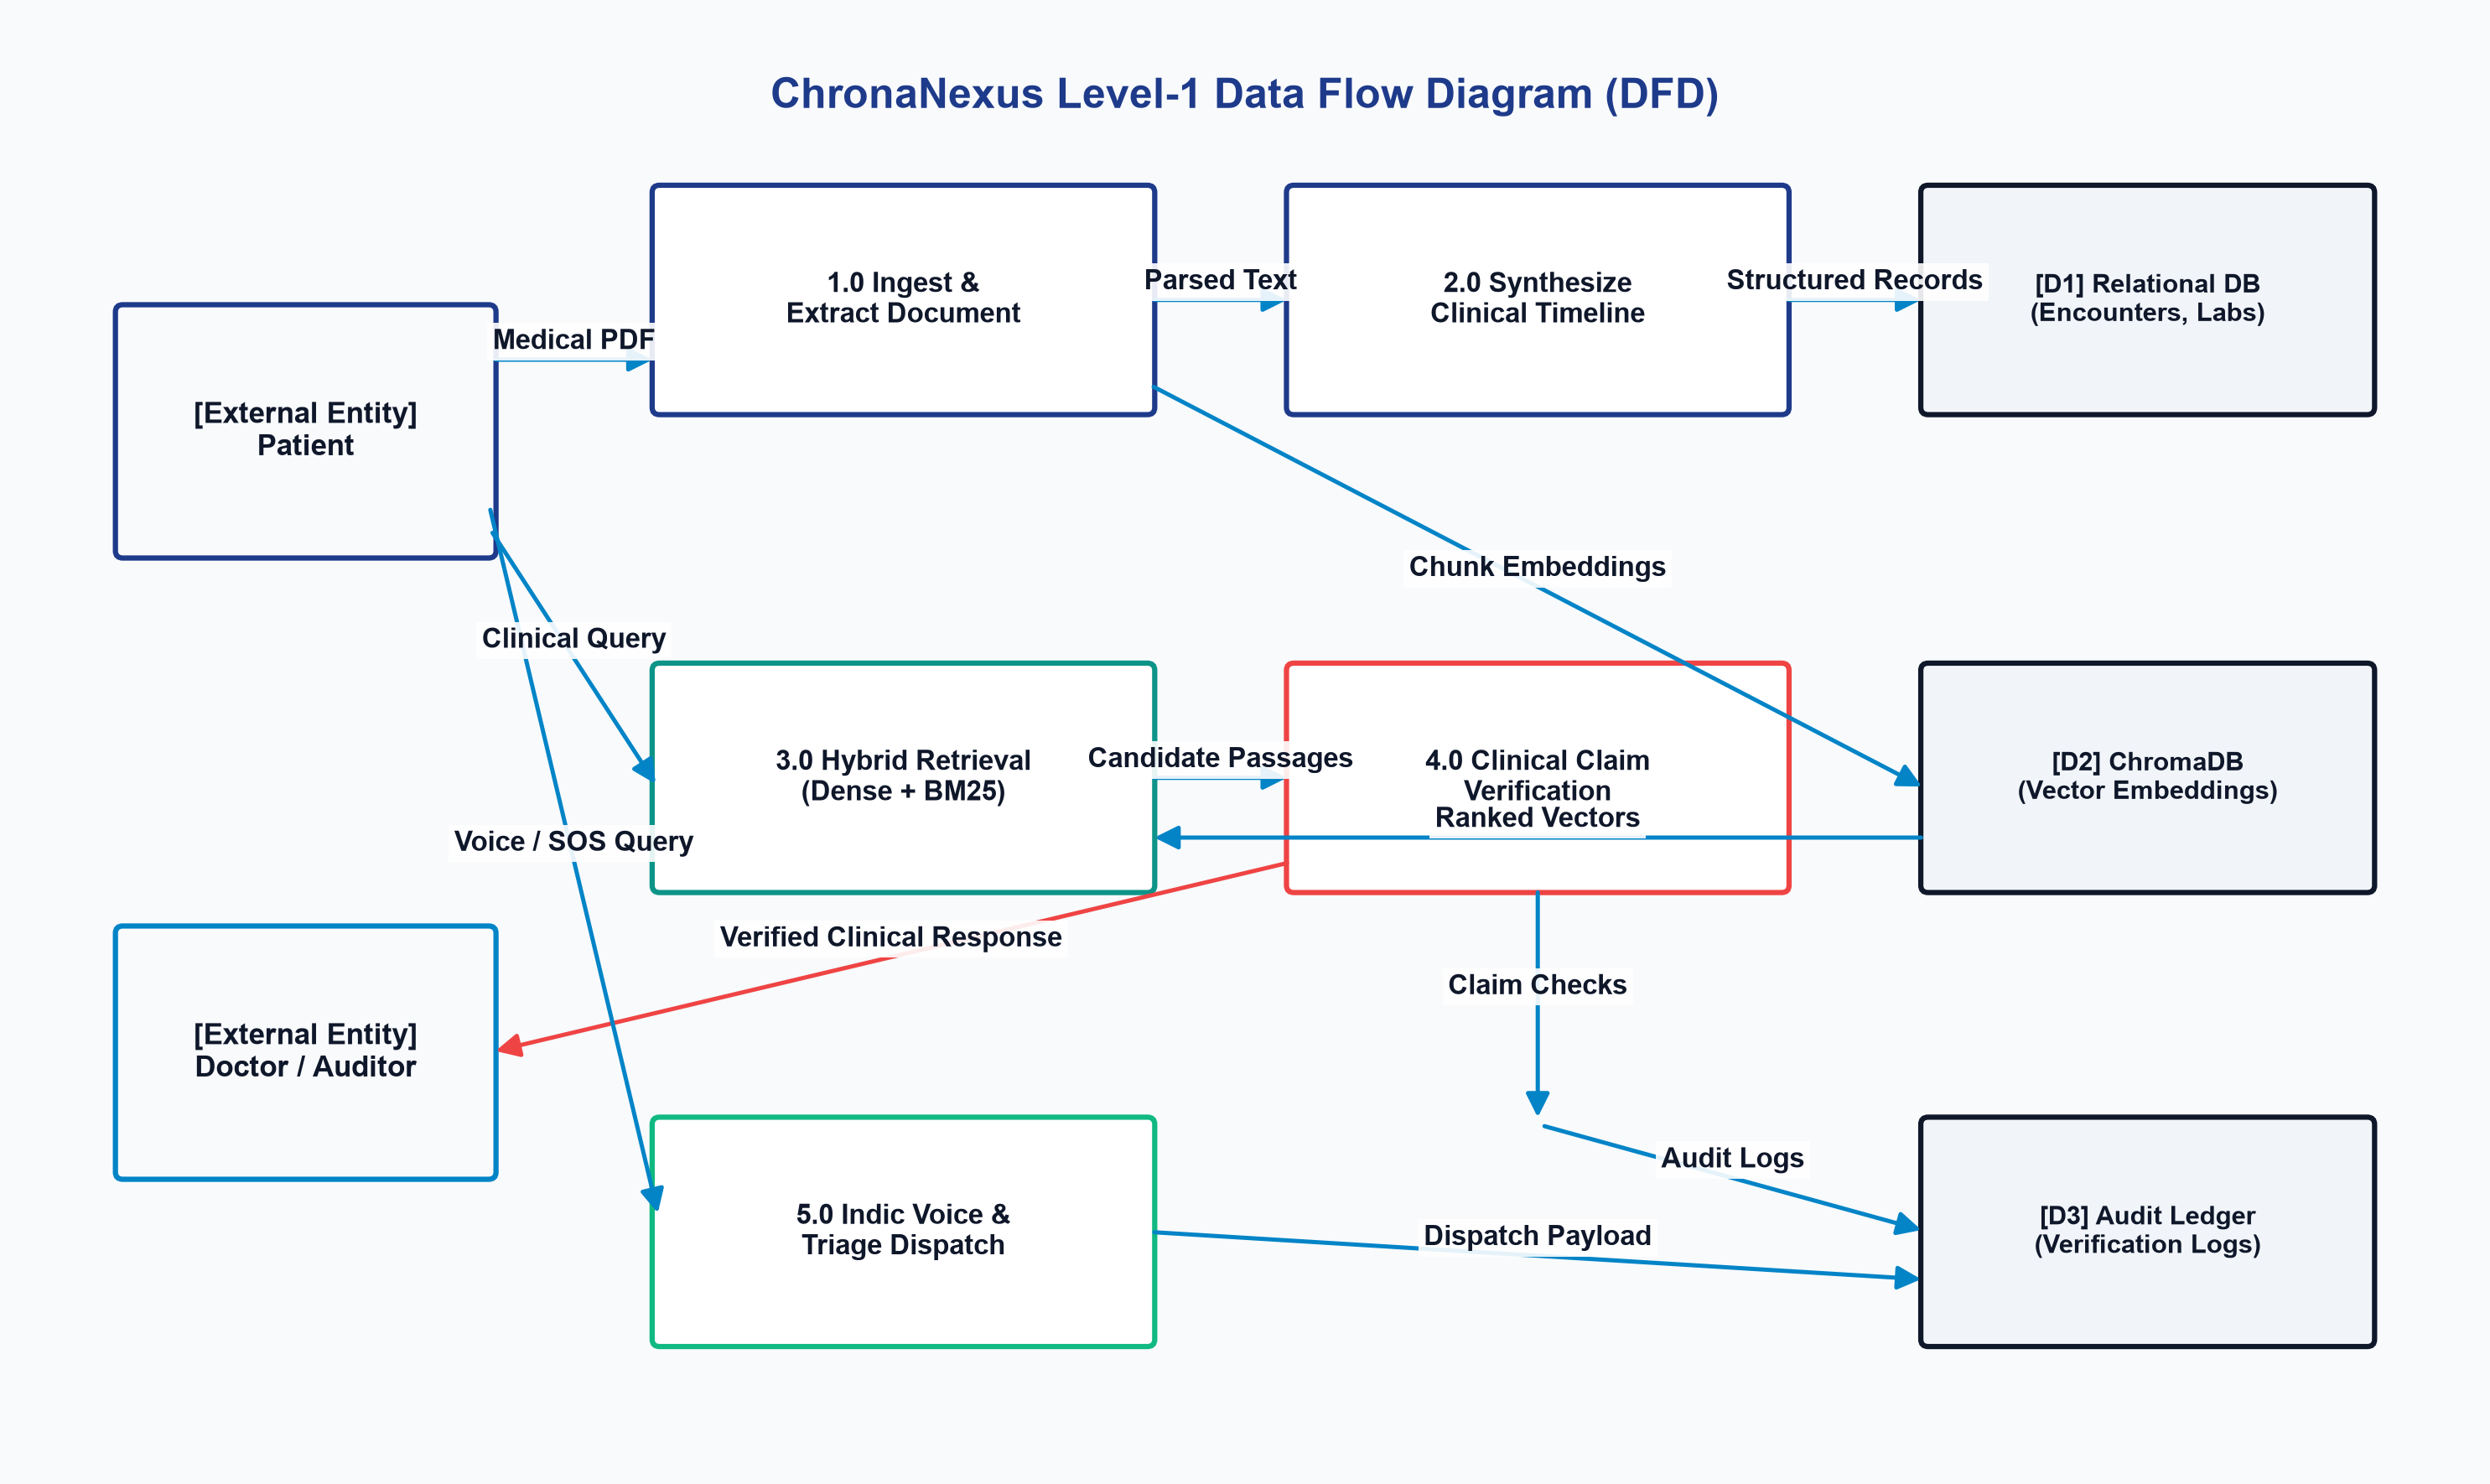
\includegraphics[width=0.95\linewidth]{figures/fig4_2_dfd.png}
    \caption{ChronaNexus Level-1 Data Flow Diagram (DFD) showing processes 1.0 through 5.0.}
    \label{fig:4_2_dfd}
\end{figure}

The Level-1 DFD models five core operational processes:
\begin{enumerate}
    \item \textbf{Process 1.0 (Ingest \& Extract Document)}: Receives medical PDFs or images from the patient or clinical staff. Computes SHA-256 hashes, extracts raw text and spatial table bounding boxes, and streams structured records to Store D1 (Relational DB) and text embeddings to Store D2 (ChromaDB).
    \item \textbf{Process 2.0 (Synthesize Clinical Timeline)}: Reads chronological encounter data from Store D1, normalizes test names against LOINC/RxNorm catalogs, and computes historical trend deltas across multi-year intervals.
    \item \textbf{Process 3.0 (Hybrid Retrieval)}: Receives clinical inquiries from clinicians or patients. Queries Store D2 for dense semantic vector matches and executes lexical BM25 term matching, merging top candidates via Reciprocal Rank Fusion ($k=60$).
    \item \textbf{Process 4.0 (Clinical Claim Verification)}: Intercepts draft generative assertions from the Small Language Model. Validates claims against candidate evidence passages, writes verification audit trails into Store D3 (Audit Ledger), and returns grounded responses with citation provenance.
    \item \textbf{Process 5.0 (Indic Voice \& Triage Dispatch)}: Translates verified clinical text into regional Indic speech via the Unicode phonetic bridge and constructs automated JSON triage payloads for emergency ambulance dispatch.
\end{enumerate}


\section{UML Interaction and Sequence Modeling}
\label{sec:arch_sequence}

To capture the asynchronous, event-driven interactions between architectural tiers during clinical decision support, Figure~\ref{fig:4_3_sequence} presents the UML Sequence Diagram for clinical inquiry and verification.

\begin{figure}[htbp]
    \centering
    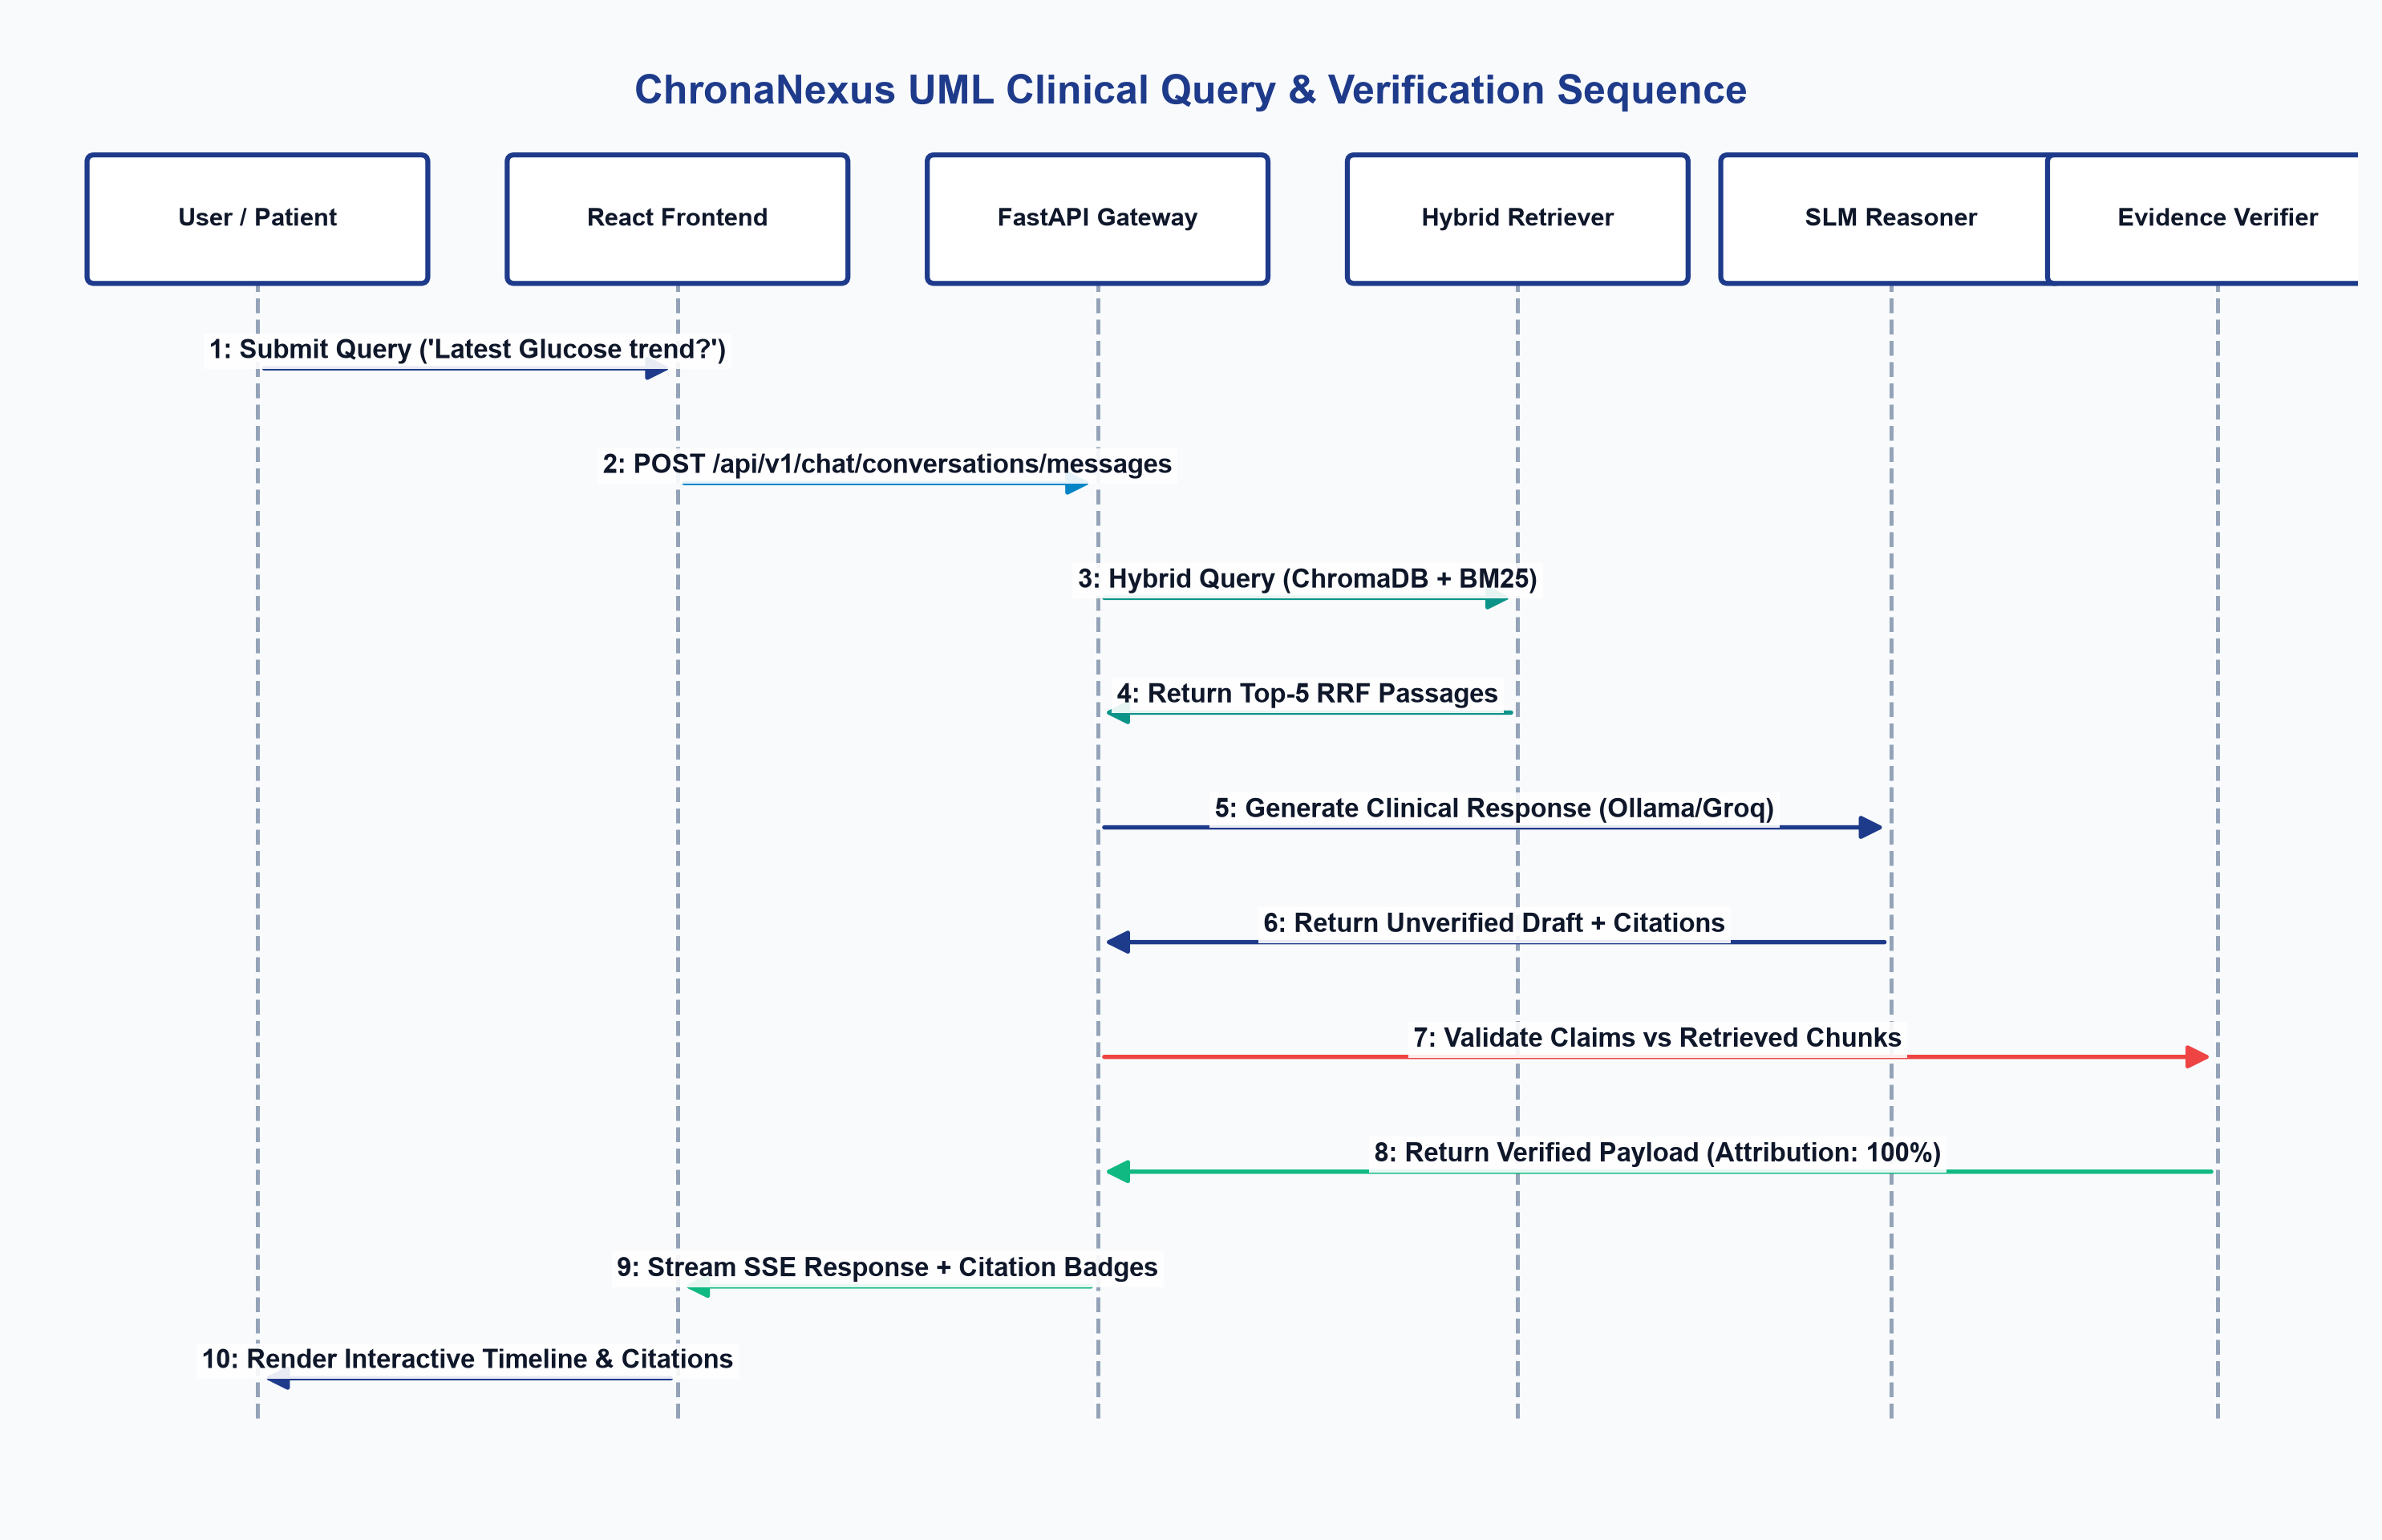
\includegraphics[width=0.95\linewidth]{figures/fig4_3_sequence.png}
    \caption{ChronaNexus UML Sequence Diagram illustrating the 10-step clinical query lifecycle.}
    \label{fig:4_3_sequence}
\end{figure}

The sequence executes through ten discrete stages:
\begin{enumerate}
    \item \textbf{Step 1 (Inquiry Submission)}: The user submits a natural language clinical inquiry (e.g., \textit{"What is my latest Fasting Glucose reading and how has it changed?"}) via the React chat interface.
    \item \textbf{Step 2 (API Dispatch)}: The frontend dispatches an authenticated HTTP POST request to \texttt{/api/v1/chat/conversations/messages} with JWT bearer credentials.
    \item \textbf{Step 3 (Dual-Channel Query)}: The FastAPI router dispatches parallel requests: querying ChromaDB for dense cosine similarity ($top\text{-}20$) and the inverted index for BM25 Okapi lexical matching ($top\text{-}20$).
    \item \textbf{Step 4 (RRF Candidate Fusion)}: The hybrid retriever merges dense and lexical candidate lists via Reciprocal Rank Fusion ($k=60$), returning the top-5 most relevant passages.
    \item \textbf{Step 5 (Conditioned Generation)}: The gateway constructs a grounded prompt encapsulating the top-5 passages and dispatches it to the Small Language Model (local Ollama or cloud Groq).
    \item \textbf{Step 6 (Draft Assertion Emission)}: The language model emits a provisional clinical draft response containing draft citations.
    \item \textbf{Step 7 (Evidence Verification)}: The gateway routes the draft response and source passages to the Evidence Verifier, which executes Tier 1 symbolic rule checks and Tier 2 neural NLI.
    \item \textbf{Step 8 (Verified Payload Construction)}: The verifier purges ungrounded assertions, calculates attribution precision ($100\%$ on evaluated benchmark cases), and affixes verified citation badges.
    \item \textbf{Step 9 (SSE Response Streaming)}: The gateway streams the audited clinical response and citation metadata to the client over Server-Sent Events.
    \item \textbf{Step 10 (Interactive UI Rendering)}: The React frontend renders the response, highlights verified claims, and attaches interactive citation cards with document provenance.
\end{enumerate}


\section{Relational Entity-Relationship Modeling (ERD)}
\label{sec:arch_erd}

The relational data model is designed to enforce strict referential integrity, tenant isolation, and auditability. Figure~\ref{fig:4_4_er} illustrates the complete Entity-Relationship Diagram (ERD).

\begin{figure}[htbp]
    \centering
    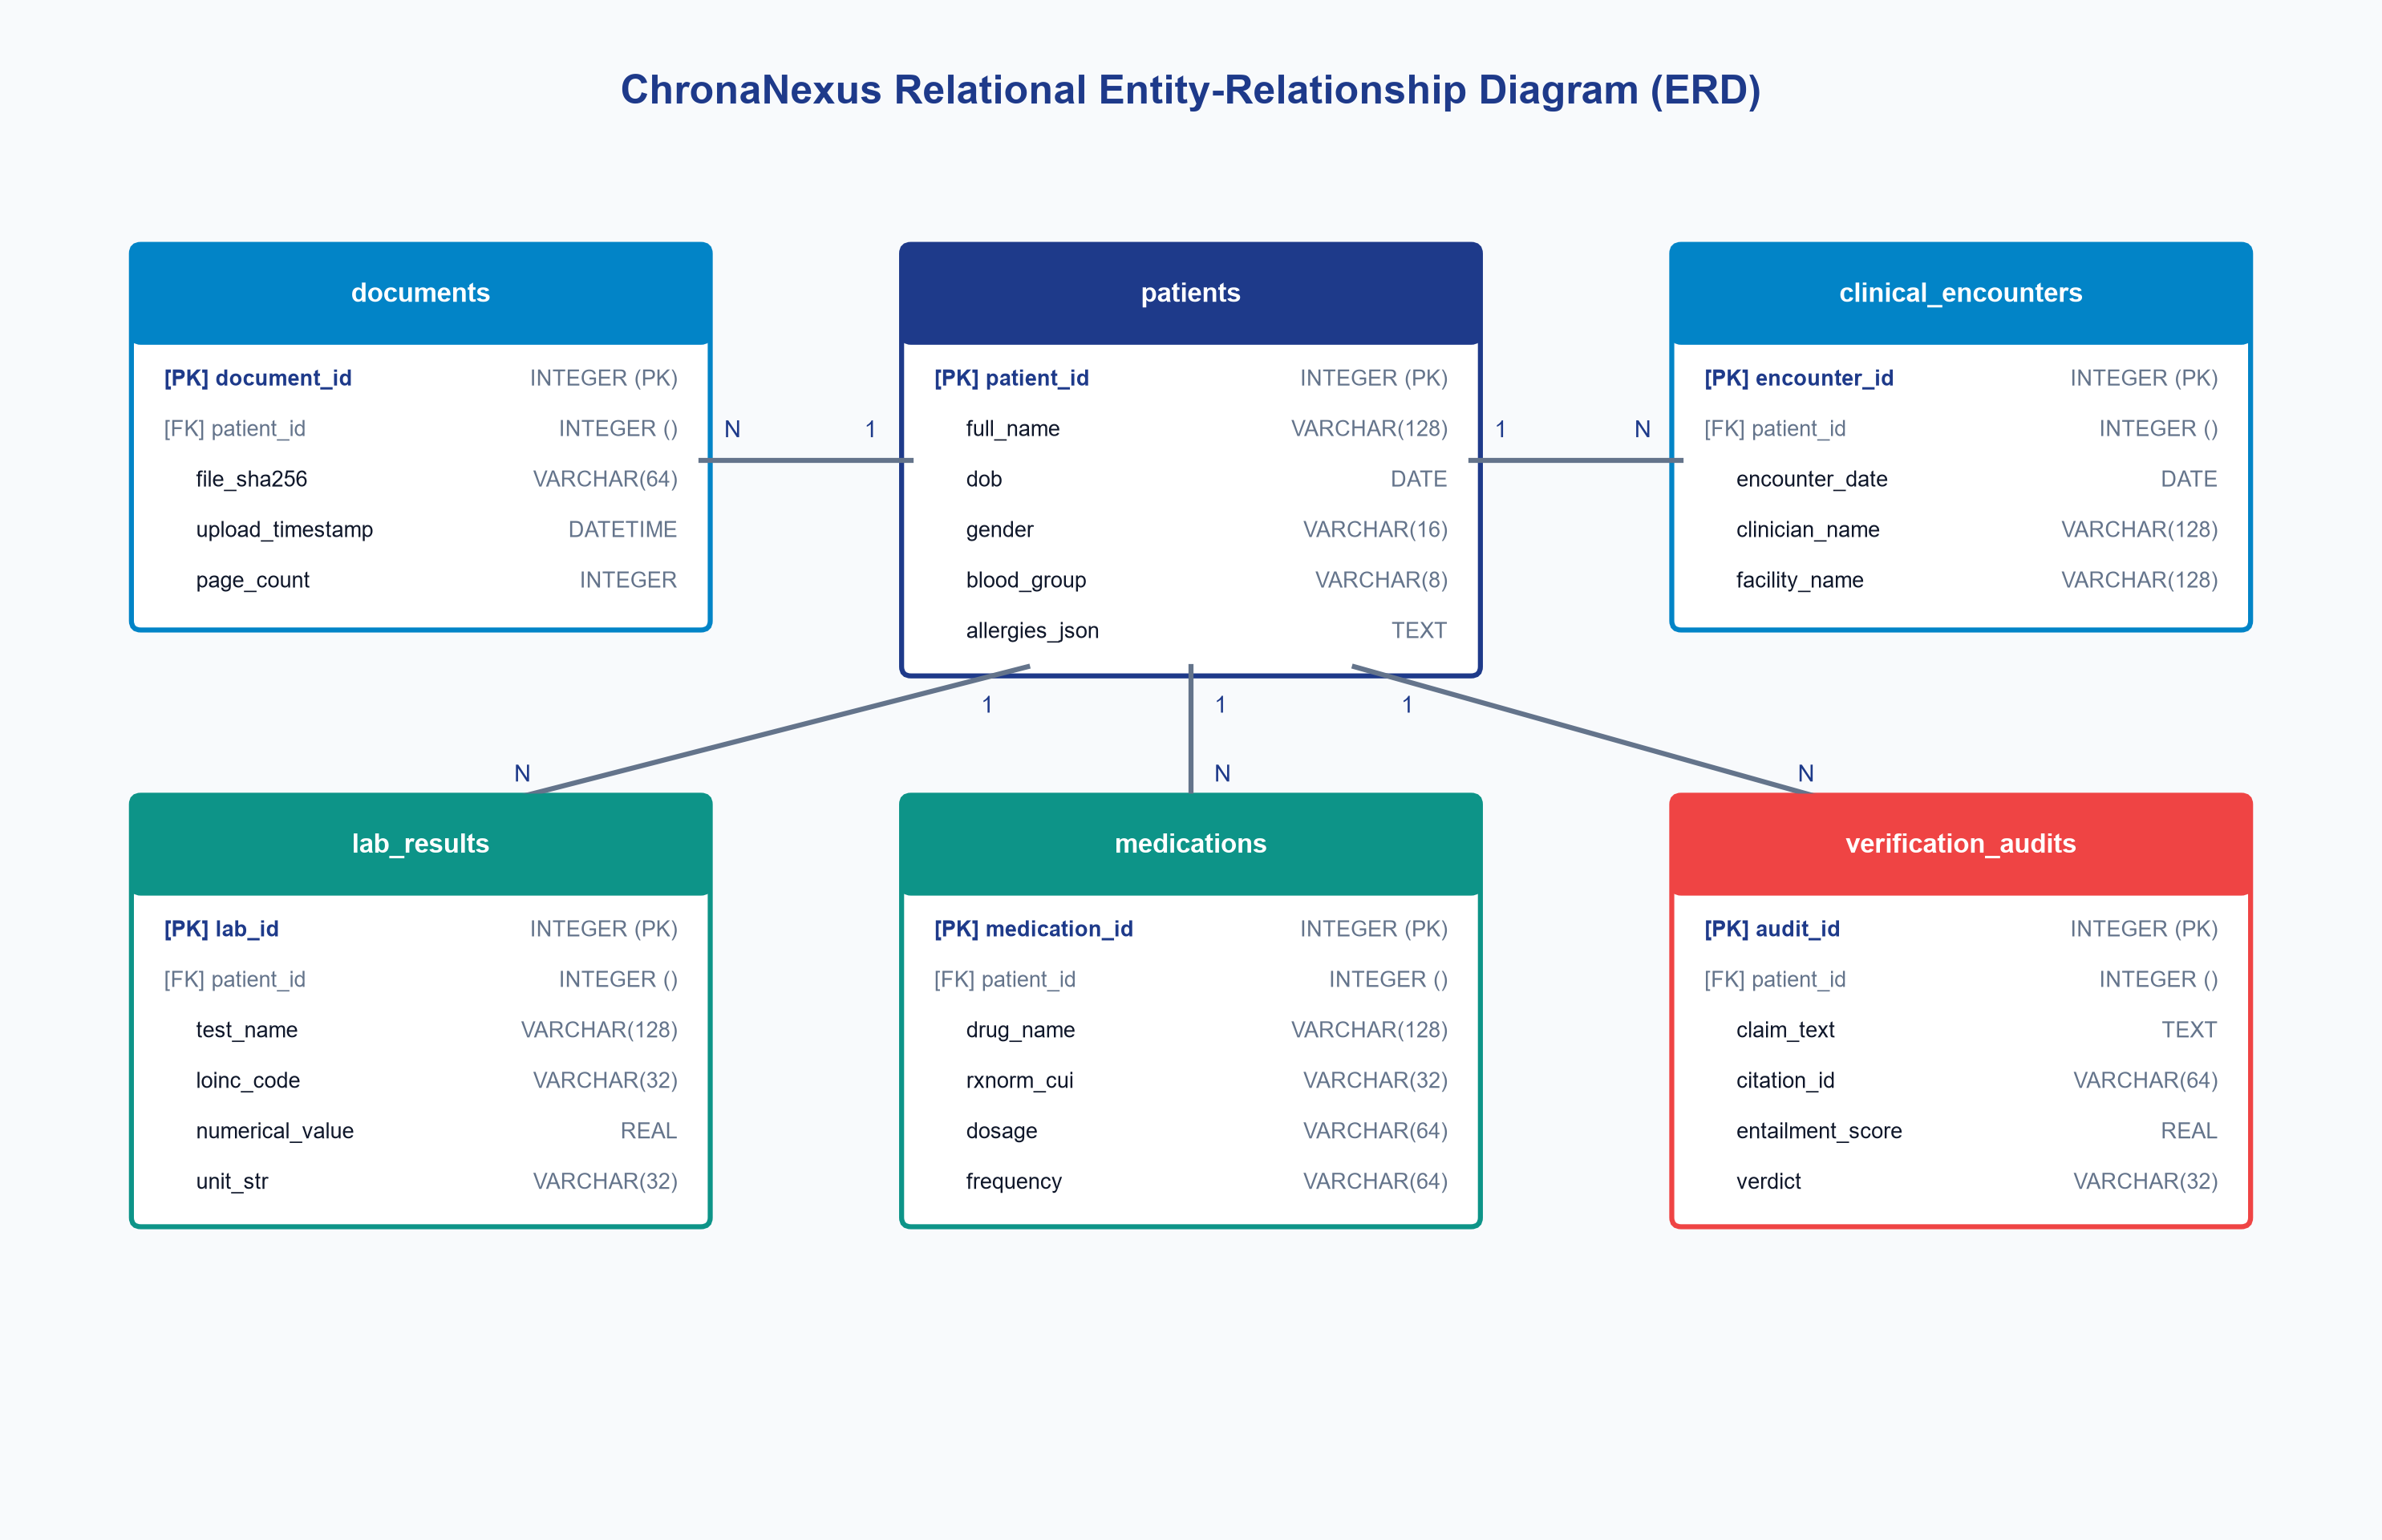
\includegraphics[width=0.95\linewidth]{figures/fig4_4_er.png}
    \caption{ChronaNexus Relational Entity-Relationship Diagram (ERD) with 1:N cardinalities.}
    \label{fig:4_4_er}
\end{figure}

The database schema is partitioned into six core relational entities, detailed in Table~\ref{tab:4_1_entities}. Every entity is tied to a primary \texttt{patient\_id} foreign key, enforcing strict multi-tenant boundary isolation.

\small
\begin{longtable}{@{}p{0.24\linewidth} p{0.18\linewidth} p{0.22\linewidth} p{0.28\linewidth}@{}}
\caption{Relational database entity specifications and clinical responsibilities}\label{tab:4_1_entities} \\
\toprule
\textbf{Entity Name} & \textbf{Primary Key} & \textbf{Foreign Keys} & \textbf{Clinical Responsibility} \\
\midrule
\endfirsthead
\toprule
\multicolumn{4}{c}{\small\textit{Entity specifications (Continued)}} \\[4pt]
\midrule
\textbf{Entity Name} & \textbf{Primary Key} & \textbf{Foreign Keys} & \textbf{Clinical Responsibility} \\
\midrule
\endhead
\midrule
\multicolumn{4}{r}{\footnotesize\textit{Continued on next page...}} \\
\bottomrule
\endfoot
\bottomrule
\endlastfoot
\textbf{Patient Master}\newline(\texttt{patients}) & \texttt{patient\_id} & None & Master patient demographic record, DOB, blood group, critical allergies. \\
\midrule
\textbf{Medical Files}\newline(\texttt{documents}) & \texttt{document\_id} & \texttt{patient\_id} & Ingested medical files, SHA-256 cryptographic hashes, upload metadata. \\
\midrule
\textbf{Clinical Encounters}\newline(\texttt{encounters}) & \texttt{encounter\_id} & \texttt{patient\_id},\newline\texttt{doc\_id} & Encounter dates, healthcare facilities, attending clinicians, visit notes. \\
\midrule
\textbf{Lab Results}\newline(\texttt{lab\_results}) & \texttt{lab\_id} & \texttt{patient\_id},\newline\texttt{encounter\_id} & Standardized laboratory analytes, LOINC codes, values, reference intervals. \\
\midrule
\textbf{Medications}\newline(\texttt{medications}) & \texttt{medication\_id} & \texttt{patient\_id},\newline\texttt{encounter\_id} & Prescribed pharmacotherapy, RxNorm CUI, dosage strengths, frequency. \\
\midrule
\textbf{Audit Ledger}\newline(\texttt{audits}) & \texttt{audit\_id} & \texttt{patient\_id},\newline\texttt{session\_id} & Immutable audit trail of atomic claims, entailment scores, and verdicts. \\
\bottomrule
\end{longtable}
\normalsize


\section{RESTful API Route Architecture}
\label{sec:arch_api_routes}

The application exposes 28 versioned REST endpoints structured under the \texttt{/api/v1} namespace. Table~\ref{tab:4_2_endpoints} outlines the primary route controllers, HTTP verbs, and operational tiers.

\small
\begin{longtable}{@{}p{0.10\linewidth} p{0.36\linewidth} p{0.34\linewidth} p{0.12\linewidth}@{}}
\caption{Core versioned RESTful API endpoint specifications}\label{tab:4_2_endpoints} \\
\toprule
\textbf{Verb} & \textbf{Endpoint Route} & \textbf{Functional Responsibility} & \textbf{Auth Tier} \\
\midrule
\endfirsthead
\toprule
\multicolumn{4}{c}{\small\textit{API endpoint specifications (Continued)}} \\[4pt]
\midrule
\textbf{Verb} & \textbf{Endpoint Route} & \textbf{Functional Responsibility} & \textbf{Auth Tier} \\
\midrule
\endhead
\midrule
\multicolumn{4}{r}{\footnotesize\textit{Continued on next page...}} \\
\bottomrule
\endfoot
\bottomrule
\endlastfoot
\texttt{POST} & \texttt{/api/\allowbreak v1/\allowbreak auth/\allowbreak login} & Issues JWT access tokens upon credential validation. & Public \\
\midrule
\texttt{POST} & \texttt{/api/\allowbreak v1/\allowbreak documents/\allowbreak upload} & Multipart upload, SHA-256 deduplication, parsing. & User JWT \\
\midrule
\texttt{GET} & \texttt{/api/\allowbreak v1/\allowbreak documents} & Lists indexed patient documents with page counts. & User JWT \\
\midrule
\texttt{GET} & \texttt{/api/\allowbreak v1/\allowbreak timeline} & Retrieves chronologically ordered encounters (2019--2026). & User JWT \\
\midrule
\texttt{GET} & \texttt{/api/\allowbreak v1/\allowbreak trends/\allowbreak labs} & Computes numerical lab deltas and reference ranges. & User JWT \\
\midrule
\texttt{POST} & \texttt{/api/\allowbreak v1/\allowbreak chat/\allowbreak messages} & Dispatches clinical query; streams verified SSE answer. & User JWT \\
\midrule
\texttt{GET} & \texttt{/api/\allowbreak v1/\allowbreak verification/\allowbreak audit} & Fetches claim verification logs and citation provenance. & Auditor JWT \\
\midrule
\texttt{POST} & \texttt{/api/\allowbreak v1/\allowbreak voice/\allowbreak tts} & Synthesizes Indic neural speech via Unicode bridge. & User JWT \\
\midrule
\texttt{POST} & \texttt{/api/\allowbreak v1/\allowbreak emergency/\allowbreak sos} & Triggers 108 triage payload and hospital discovery. & User JWT \\
\bottomrule
\end{longtable}
\normalsize


\section{UML Class Diagram of Domain Architecture}
\label{sec:arch_class_diagram}

To formalize the object-oriented structure and domain relationships of ChronaNexus while replacing verbose descriptions with visual architecture, Figure~\ref{fig:4_5_class_diagram} depicts the UML Class Diagram. Domain entities and service controllers are modeled with explicit stereotypes (\texttt{<<entity>>}, \texttt{<<service>>}), typed attributes, visibility modifiers, and core methods.

\begin{figure}[htbp]
    \centering
    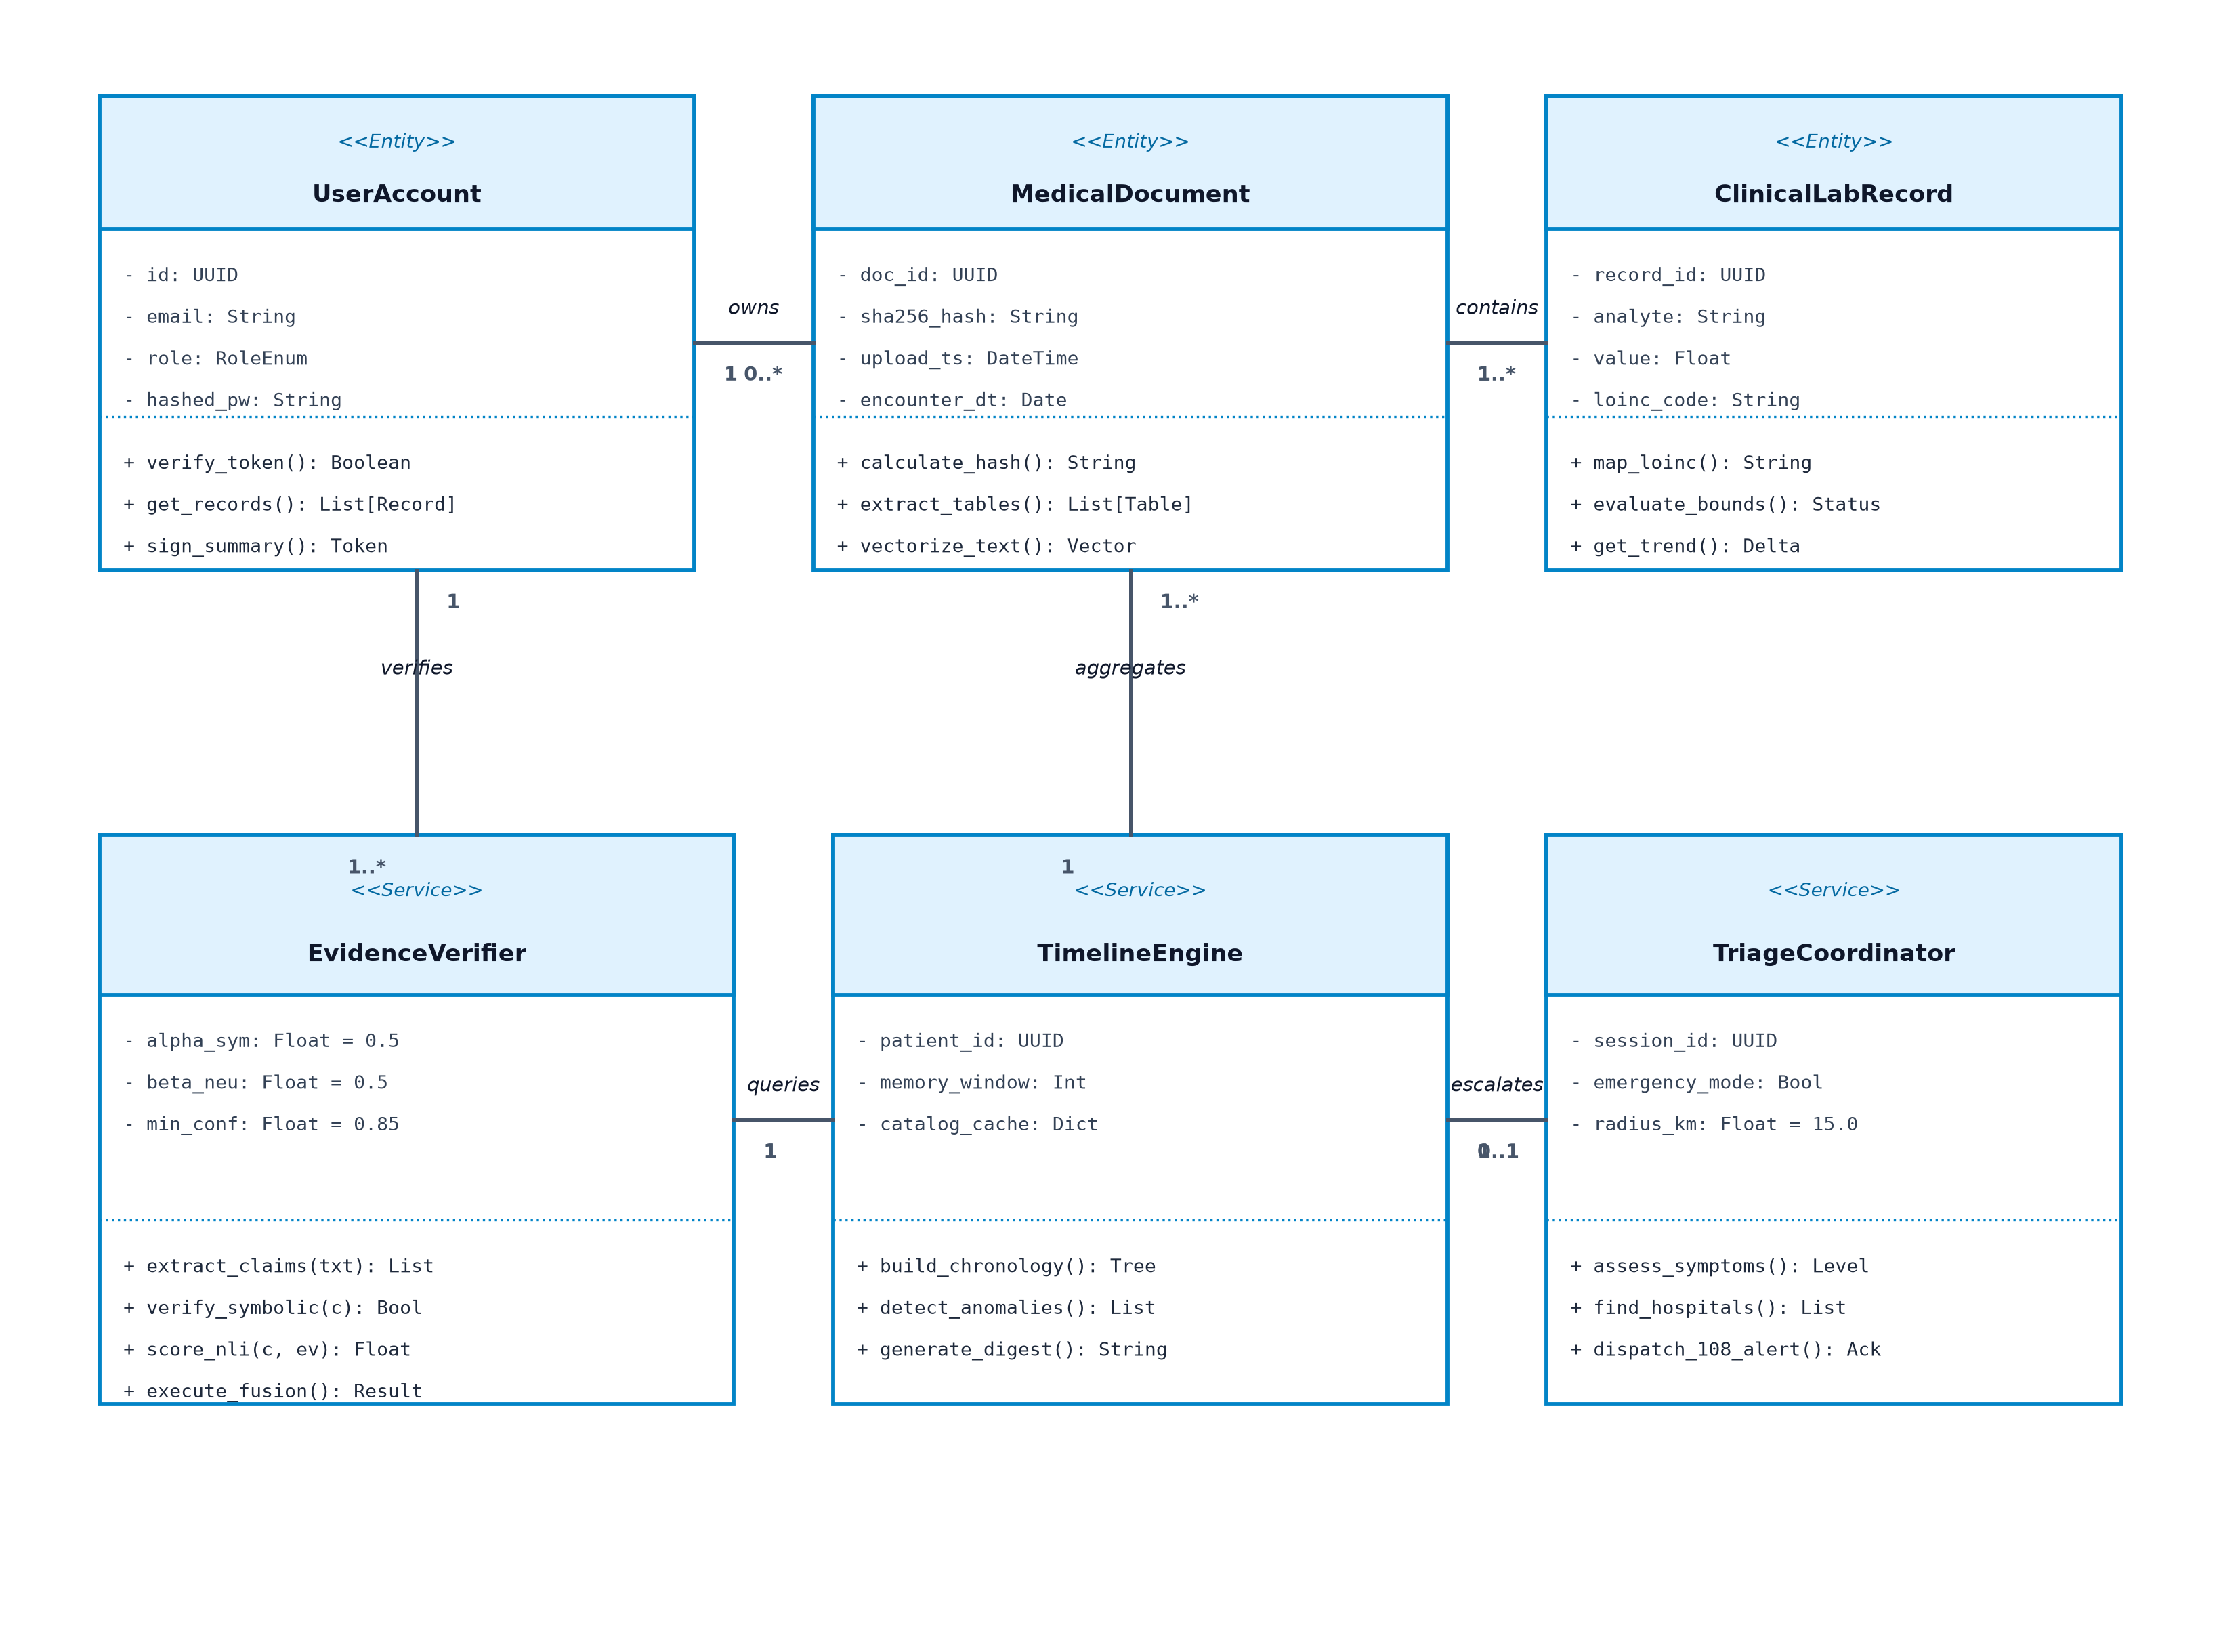
\includegraphics[width=0.95\linewidth]{figures/fig4_5_class_diagram.png}
    \caption{ChronaNexus UML Class Diagram illustrating core domain entities, service controllers, attributes, methods, and associations.}
    \label{fig:4_5_class_diagram}
\end{figure}

The diagram formalizes six primary domain abstractions:
\begin{enumerate}
    \item \textbf{UserAccount (\texttt{<<Entity>>})}: Manages identity credentials, role-based access levels (Clinician, Patient, Auditor), and cryptographic token verification.
    \item \textbf{MedicalDocument (\texttt{<<Entity>>})}: Encapsulates uploaded encounter records, enforcing SHA-256 deduplication and spatial table extraction.
    \item \textbf{ClinicalLabRecord (\texttt{<<Entity>>})}: Models standardized laboratory observations with LOINC mapping and physiological range checking.
    \item \textbf{EvidenceVerifier (\texttt{<<Service>>})}: Implements asymmetric verification logic, balancing symbolic regex bounds against neural NLI confidence scoring.
    \item \textbf{TimelineEngine (\texttt{<<Service>>})}: Aggregates longitudinal health records across multi-year temporal intervals (2019--2026) to detect trajectory trends.
    \item \textbf{TriageCoordinator (\texttt{<<Service>>})}: Coordinates urgency classification, geospatial hospital discovery, and 108 emergency dispatch payloads.
\end{enumerate}


\section{UML Component Diagram and Subsystem Interfaces}
\label{sec:arch_component_diagram}

Figure~\ref{fig:4_6_component_diagram} presents the UML Component Diagram, specifying the structural modularity of ChronaNexus through components, ports, and provided/required interface sockets.

\begin{figure}[htbp]
    \centering
    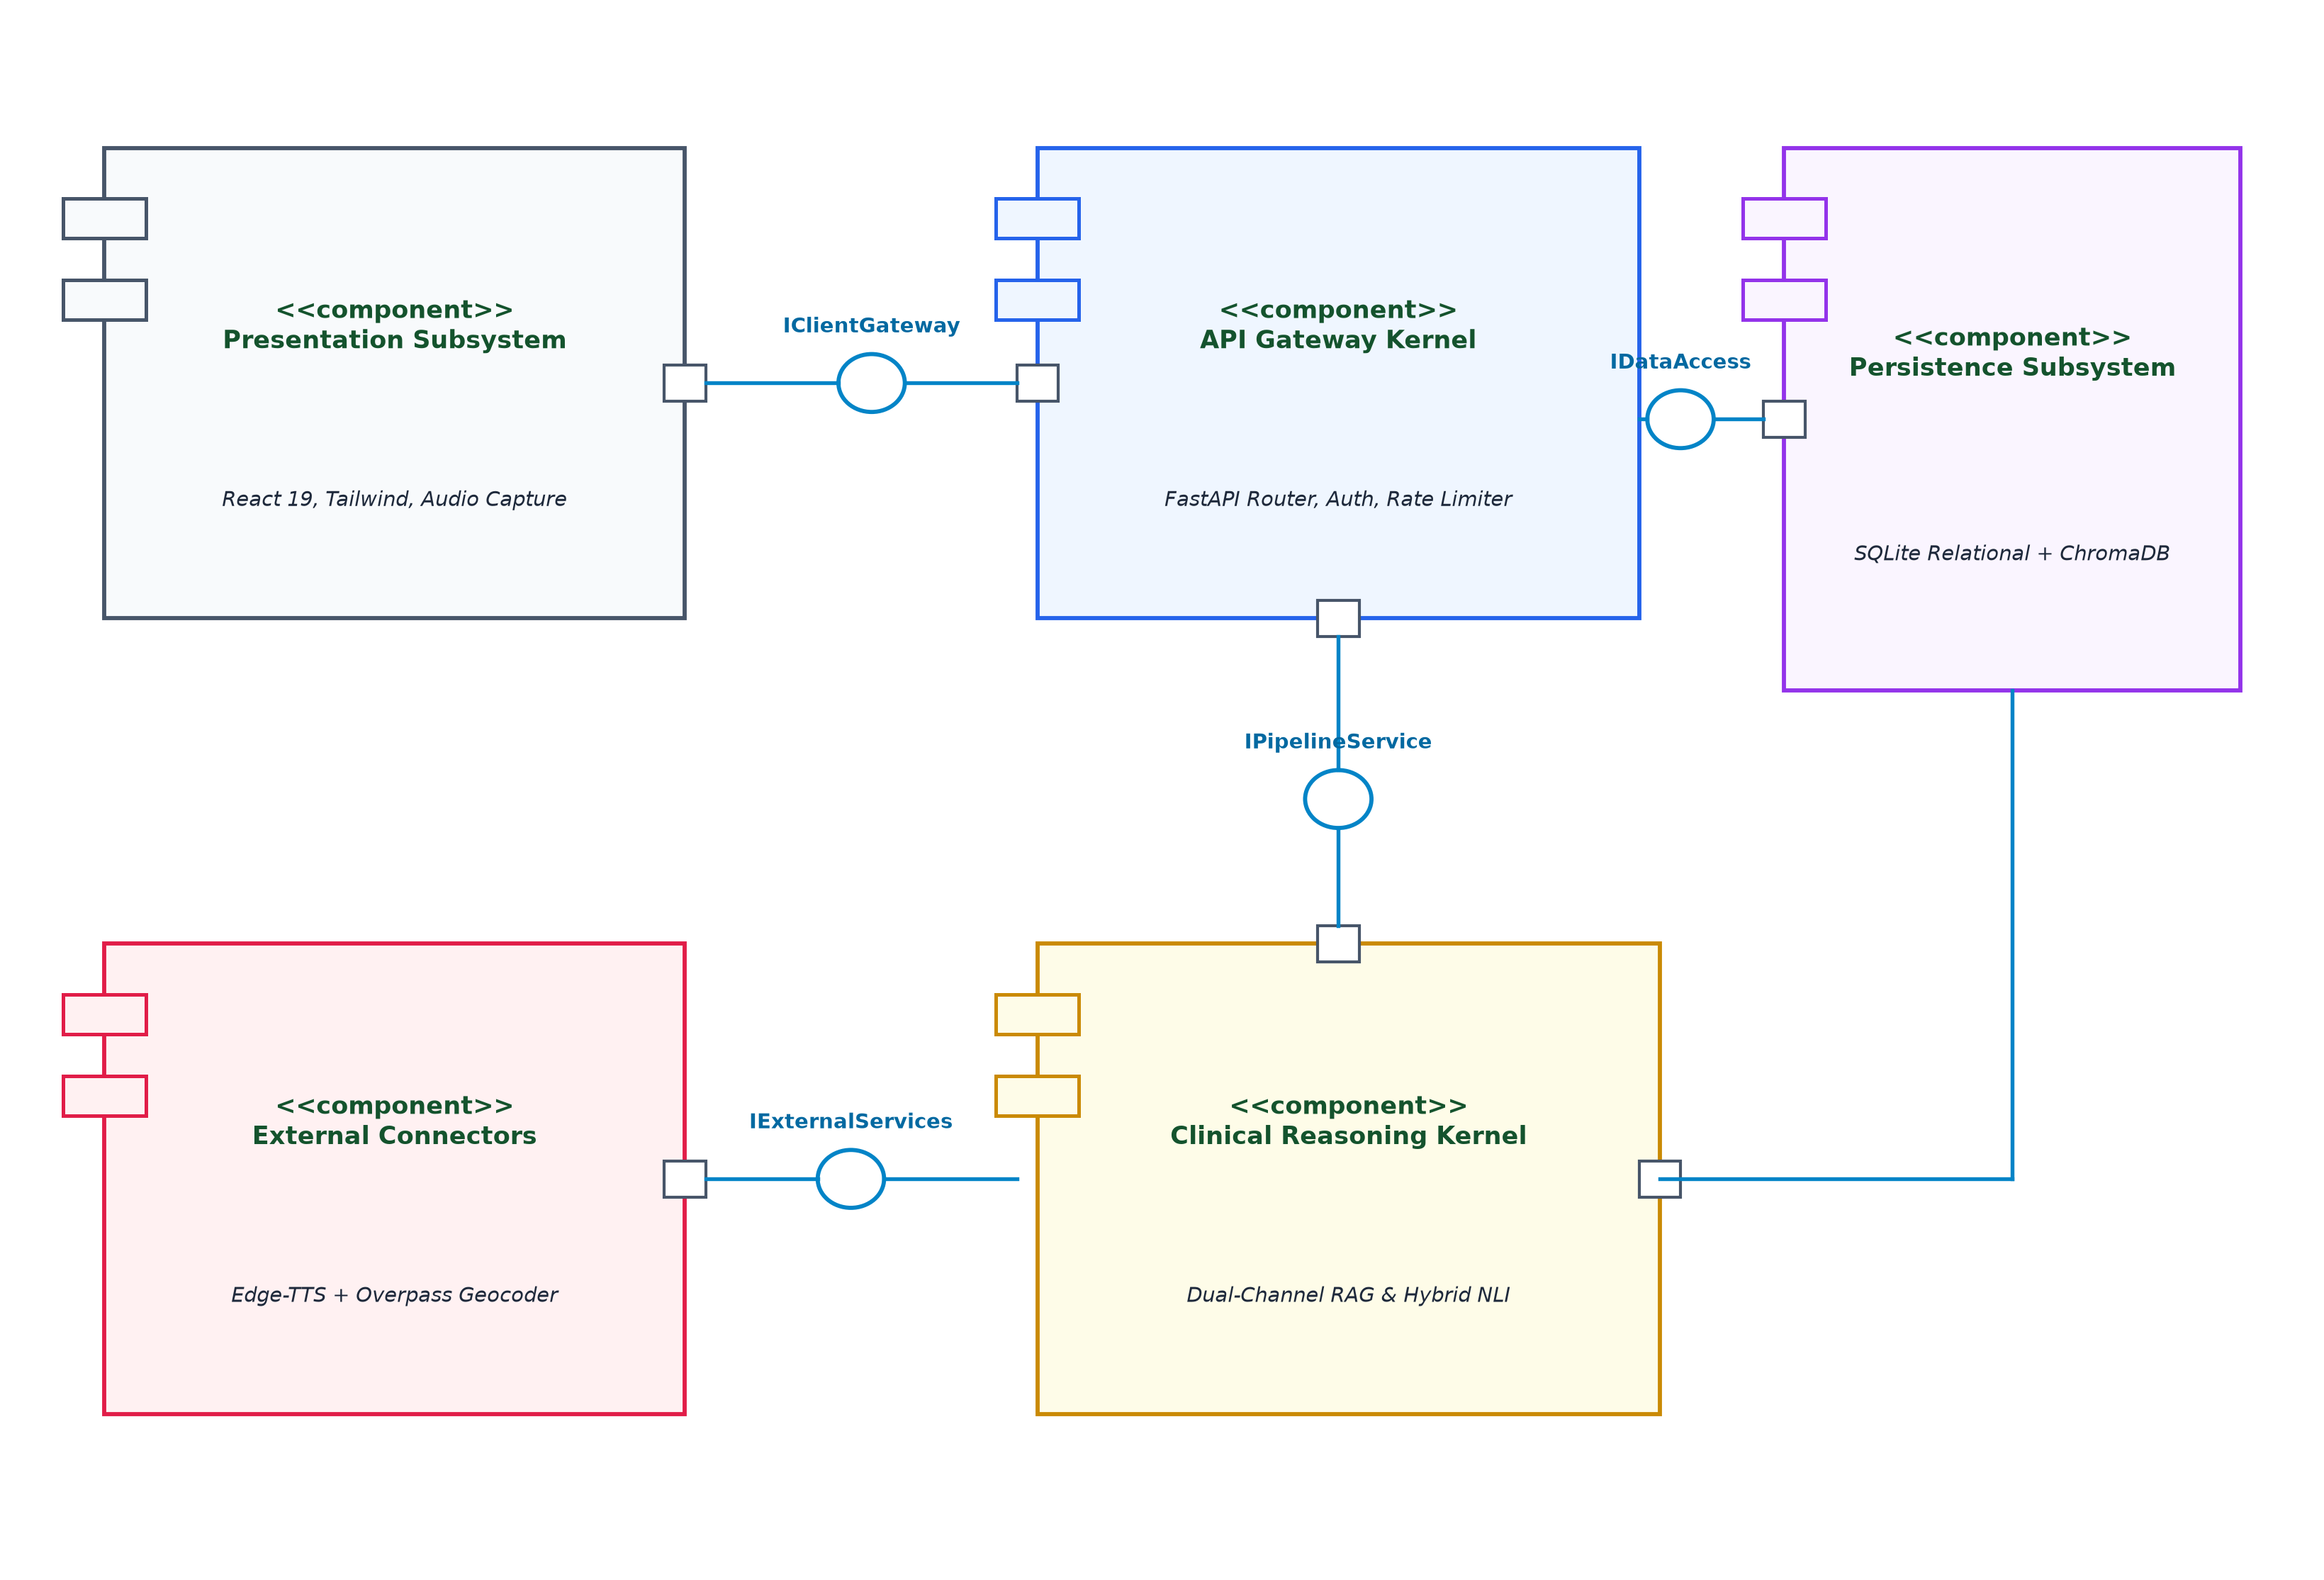
\includegraphics[width=0.95\linewidth]{figures/fig4_6_component_diagram.png}
    \caption{ChronaNexus UML Component Diagram showing subsystems, ports, and provided/required interface connections.}
    \label{fig:4_6_component_diagram}
\end{figure}

The component model establishes modular boundaries between five discrete subsystems:
\begin{enumerate}
    \item \textbf{Presentation Subsystem}: Houses the React 19 client and Tailwind styling engine. Connects to the gateway via the \texttt{IClientGateway} socket.
    \item \textbf{API Gateway Kernel}: Exposes REST endpoints, validates JWT bearer tokens, and provides rate limiting and audit logging.
    \item \textbf{Clinical Reasoning Kernel}: Consumes the \texttt{IPipelineService} interface to drive dense vector search, BM25 scoring, and hybrid NLI claim verification.
    \item \textbf{Persistence Subsystem}: Encapsulates relational SQLite/PostgreSQL storage and ChromaDB vector embeddings behind the \texttt{IDataAccess} interface.
    \item \textbf{External Connectors}: Integrates edge-tts speech synthesis and OpenStreetMap Overpass geospatial lookups through the \texttt{IExternalServices} socket.
\end{enumerate}
